\documentclass{article}
\usepackage[margin=1in]{geometry}
\usepackage{tabulary}
\usepackage{float}
\usepackage{lipsum}
\usepackage[utf8]{inputenc}
\usepackage{hyperref}
\usepackage{graphicx}
\usepackage{graphics}
\usepackage{listings}
\lstset
{ %Formatting for code in appendix
    language=C,
    basicstyle=\small,
    numbers=left,
    stepnumber=1,
    showstringspaces=false,
    tabsize=1,
    breaklines=true,
    breakatwhitespace=false,
}
\usepackage{xcolor}
\lstset{escapeinside={<@}{@>}}
\usepackage[T1]{fontenc}
\usepackage[parfill]{parskip}
\newcommand{\code}[1]{\textsf{#1}}
\setlength{\parindent}{0em}
\begin{document}
\begin{center}{\LARGE CS406: Compilers} \end{center}
\begin{center}{\large Programming Assignment 3: Symbol Table,  Due: 4/3/2020} \end{center}

\bigskip



\section{Introduction}
Your goal in this step is to process variable declarations and create a Symbol Table. 
A symbol table is a data structure that keeps information about non-keyword symbols that appear in source programs. 
Variables and function names are examples of such symbols. 
The symbols added to the symbol table will be used in many of the further phases of the compilation.
In the previous assignment you didn't need token values since only token types are used by parser generator tools to guide parsing. 
But in this assignment your parser needs to get token values such as identifier names and string literals from your scanner. 
You also need to add semantic actions to create symbol table entries and add those to the symbol table.


\section{Background}
\subsection{Semantic Actions}
Semantic actions are steps that your compiler takes as the parser recognizes constructs in your program. 
Another way to think about this is that semantic actions are code that executes as your compiler matches various parts of the program (constructs like {\em variable declarations} or tokens like {\em identifiers}). 
By taking the right kind of action when the right kind of construct is recognized, you can make your compiler do useful work!

\texttt{STRING foo := "Hello World";}

Which produces the (partial) parse tree below:

\begin{figure}[H]
	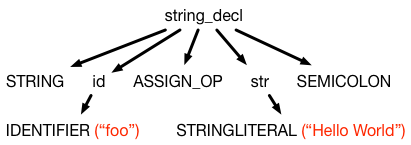
\includegraphics[scale=0.5]{parsetree}
\end{figure}

We can create {\em semantic records} for each of the tokens \texttt{IDENTIFIER} and \texttt{STRINGLITERAL} that record their values (``foo'' and ``Hello World'', respectively), and ``pass them up'' the tree so that those records are the records for \texttt{id} and \texttt{str}. We can then construct a semantic record for \texttt{string\_decl} using the semantic records of its children to produce a structure that captures the necessary information for a string declaration entry in your symbol table (and even add the entry to the symbol table).

\subsubsection{Parser-driven Semantic Actions}
It may seem like a lot of work to keep track of pieces of data at each node of the parse tree and assemble them into more complicated records. But most parsers help do this {\em automatically}. 
As they build up the parse tree, they will call actions that execute to collect data from the parse tree and create semantic records. 
In essence, the parsers perform a {\em post-order} traversal of the parse tree as {\em they walk the tree}, and store information about the necessary semantic records in a way that you can easily retrieve them. 
Let's look at how this works for both ANTLR and bison.

For both of these, it is worth remembering two things:
\begin{enumerate}
	\item Tokens become leaves in the parse tree. The semantic record for a token is either always the text associated with that token (if you're using ANTLR) or whatever you assign \texttt{yylval} to in your scanner (if you're using flex/bison).
	\item {\em Every} symbol that shows up in a grammar rule will be a node in your parse tree, and that if you recognize a grammar rule, there will be a node in your parse tree associated with the left-hand-side of the rule and that node will have a separate child for each of the symbols that appear on the right hand side.
\end{enumerate}

\subsubsection{ANTLR}
In ANTLR, you can put arbitrary Java code in braces (\texttt{\{\}}) at various points in the right hand side of a grammar rule in your \texttt{.g4} file; this code will execute as soon as the symbol immediately before the braces has been matched (if it's a token) or predicted and matched (if it's a non-terminal).

The ``main'' semantic action for a rule will go at the very end of the rule (in other words, it will execute once the entire rule has been matched). As part of this rule, you can assign a value to the semantic record that will be associated with the left hand side of the rule. You name the semantic record and tell ANTLR what type that record should have using a \texttt{returns} annotation.

You can then extract information from the semantic records of the children by giving variable names to the children you have matched. You can either access that child's semantic record by accessing \texttt{\$a.x} where $a is the name you gave the child and $x is the name you gave to the child's semantic record in the \texttt{returns} annotation, or you can access the characters associated with the child (useful when matching tokens) with \texttt{\$a.text}.

So suppose we wanted to return a structure called \texttt{StrEntry} from our \texttt{string\_decl} rule. It might look something like this:

\texttt{string\_decl [returns StrEntry s] : STRING id ASSIGN\_OP ex=str SEMI} \\
\texttt{   \{\$s = new StrEntry(); s.addID(\$id.text); s.addValue(\$ex.text);\} }

(Note that if you don't give a child a name (like \texttt{id} in the above example), ANTLR defaults to using the name of the token or non-terminal. If the same symbol shows up twice in a rule, you {\em must} give them names.)

\subsubsection{Bison}
In bison, you can put arbitrary C (or C++) code in braces at various points in the right hand side of a grammar rule in your \texttt{.y} file. It works very similarly to ANTLR in that respect. The key different in bison is understanding how to pass data around.

To set the type of a semantic record for a non-terminal, you use a \texttt{\%type} command:

\begin{lstlisting}[numbers=none]
%type <s_entry> string_decl
%type <s> id str
\end{lstlisting}

All of the types that you want to use need to be part of a union that determines the possible types for yylval, which you declare in a \texttt{\%union} declaration:
\begin{lstlisting}[numbers=none]
%union{
  StrEntry * s_entry;
  string * s;
}
\end{lstlisting}

So the \texttt{\%type} commands and \texttt{\%union} command in conjunction mean that the \texttt{string\_decl} non-terminal will produce a semantic record named \texttt{s\_entry} of type \texttt{StrEntry *} and the non-terminals \texttt{id} and \texttt{str} will produce semantic records of type string \texttt{*} named \texttt{s}.

(You can also do this by making \texttt{yylval} a \texttt{struct} instead of a \texttt{union}).

Then, when building a semantic action for a rule, \texttt{\$\$} refers to the semantic record you are building for the left hand side (whose type is determined by the \texttt{\%type} command), and \texttt{\$1, \$2}, etc. refer to the semantic records for the right hand side, listed in order. So here is the equivalent action for creating a \texttt{StrEntry} object for the \texttt{str\_decl} rule:

\texttt{string\_decl : STRING id ASSIGN\_OP str SEMI \{\$\$ = new StrEntry(); \$\$->addID(\$2); \$\$->addValue(\$4);\};}


\section{Symbol Tables}
Your task in this step of the project is to construct symbol tables for each scope in your program. For each scope, construct a symbol table, then add entries to that symbol table as you see declarations. The declarations you have to handle are integer/float declarations, which should record the name and type of the variable, and string declarations, which should {\em additionally} record the value of the string. Note that typically function declarations/definitions would result in entries in the symbol table, too, but you do not have to record them for this step.

\paragraph{Nested Symbol Tables}

In this year's variant of Micro, there are multiple scopes where variables can be declared:
\begin{itemize}
	\item Variables can be declared before any functions. These are ``global'' variables, and can be accessed from any function.
	\item Variables can be declared as part of a function's parameter list. These are ``local'' to the function, and cannot be accessed by any other function.
	\item Variables can be declared at the beginning of a function body. These are ``local'' to the function as well.
	\item Variables can be declared at the beginning of a then block, an else block, or a repeat statement. These are ``local'' to the block itself. Other blocks, even in the same function, cannot access these variables.
\end{itemize}

Note that the scopes in the program are {\em nested} (function scopes are inside global scopes, and block scopes are nested inside function scopes, or each other). You will have to keep track of this nesting so that when a piece of code uses a variable named ``x'' you know which scope that variable is from.

To handle this, we suggest you to follow the implementation strategy based on hash-tables discussed in class.

\section{What you need to do}
You should define the necessary semantic actions and data structures to let you build the symbol table(s) for Micro input programs.

At the end of the parsing phase, you should print out the symbols you found.

For each symbol table in your program, use the following format:
\begin{lstlisting}[numbers=none]
  Symbol table <scope_name>
  name <var_name> type <type_name>
  name <var_name> type <type_name> value <string_value>;
  ...
\end{lstlisting}

The global scope should be named ``GLOBAL'', function scopes should be given the same name as the function name, and block scopes should be called ``BLOCK X'' where X is a counter that increments every time you see a new block scope. 
{\em Function parameters should be included as part of the function scope}.

{\em The order of declarations matters!} We expect the entries in your symbol table to appear in the same order that they appear in the original program. Keep this in mind as you design the data structures to store your symbol tables.

See the sample outputs for more complete examples of what we are looking for.

{\em CAVEAT: You may be tempted to just print declarations as you see them, rather than building an actual tree of symbol tables. While that will suffice for step 3, it will not be sufficient for later steps of the project. We strongly suggest that you build the necessary data structures since you will have to, eventually, anyway.}

\paragraph{Handling errors}
Your compiler should output the string \texttt{DECLARATION ERROR <var\_name>} if there are two declarations with the same name {\em in the same scope}.

\paragraph{Sample inputs and outputs:} \href{https://hegden.github.io/cs406/homeworks/PA3/inputs.zip}{inputs} and \href{https://hegden.github.io/cs406/homeworks/PA3/outputs.zip}{outputs}.

\section{What you need to submit}
\begin{itemize}
	\item All of the necessary code for your compiler that you wrote yourself. You do not need to include the ANTLR jar files if you are using ANTLR.
	\item A Makefile with the following targets:
		\begin{itemize}
			\item {\em compiler}: this target will build your compiler
			\item {\em clean}: this target will remove any intermediate files that were created to build the compiler
			\item {\em team}: this target will print the same team information that you printed in step 0.
		\end{itemize}

	\item A shell script (this {\em must} be written in bash) called \texttt{runme} that runs your scanner. This script should take in two arguments: first, the input file to the scanner and second, the filename where you want to put the scanner's output. You can assume that we will have run \texttt{make compiler} before running this script.
\end{itemize}

While you may create as many other directories as you would like to organize your code or any intermediate products of the compilation process, both your \texttt{Makefile} and your \texttt{runme} script should be in the root directory of your repository.

{\em Do not submit any binaries}. Your git repo should only contain source files; no products of compilation or test cases. If you have a folder named \texttt{test} in your repo, it will be deleted as part of running our test script (though the deletion won't get pushed) -- make sure no code necessary for building/running your compiler is in such a directory.

You should tag your programming assignment submission as \textsf{submission}
\end{document}
